\chapter{Experimental results}
This chapter presents the results obtained from the design, starting from functional verification of the correctness of the implementation, to synthesis and benchmarking. The entire design has been described in SystemVerilog using hierarchical modules and behavioral constructs when possible. This both helps readability and leaves to the EDA tools the freedom of performing optimizations.

Each module has been verified locally using Verilator\footnote{\url{https://www.veripool.org/wiki/verilator}} for linting and Mentor ModelSim Intel FPGA Starter Edition for simulation. Synthesis has been carried out with Synopsys Design Compiler, on the the VLSI server provided by Politecnico di Torino.

\section{Simulation}
The choice of tools mentioned above was made because one of the pros of Verilator is that it has been found to be more verbose than ModelSim when performing syntax check and lint, thus reducing the number of possible issues during compilation and simulation. Moreover, it is completely free and open source, which nicely couples with the philosophy of the LEN5 project.

ModelSim was in the end chosen as the main simulation tool, because it is much more familiar to the designer and the limited time did not allow to learn Verilator for simulation, given that it uses a completely different paradigm, based on translating HDL to C language and using testbench templates in C as well.

The following sections focus on the test strategies used for the \ac{BPU}, which is almost as important as a standalone design, and the top-level frontend.

\subsection{\acs{BPU}}
The testbench of the \ac{BPU} is based on reading branch addresses from one file, predicting the outcome and then comparing it with the correct branch resolutions coming from a second file. One clock cycle passes between the prediction and the resolution, as to simulate the execution delay, which always takes more cycles. During this time span, the \ac{PC} is fictionally increased to simulate a normal sequential fetch situation.

Given that the length of the history register in the gshare and the length of \ac{BTB} address lead to an exponential growth of the \ac{PHT} and the \ac{BTB} itself, simulations were performed using a small number of bits for these data structures and in particular the following results refer to a configuration with a 4-bit history register and a 4-bit \ac{BTB} address. The simulation is needed to verify the correctness of the design and not the prediction performances, so having fewer bits poses no issues.

In order to test the \ac{BPU} as a singular unit, without all the surrounding processor and in particular without a register file and execution units, some specific test cases have been defined, where branch results could be derived manually without actually executing the program. Loops, in particular, suit well such simple cases.

\subsubsection{Single loop}
The first test case corresponds to the following simple loop:
\begin{lstlisting}[language=C]
  for (int i = 0; i < 10; i++)
  {
    /* loop body */
  }
\end{lstlisting}
Here, the loop condition is tested ten times as true, so the branch is taken, and the last time as false, so the branch is not taken.

\begin{sidewaysfigure}[p]
  \centering
  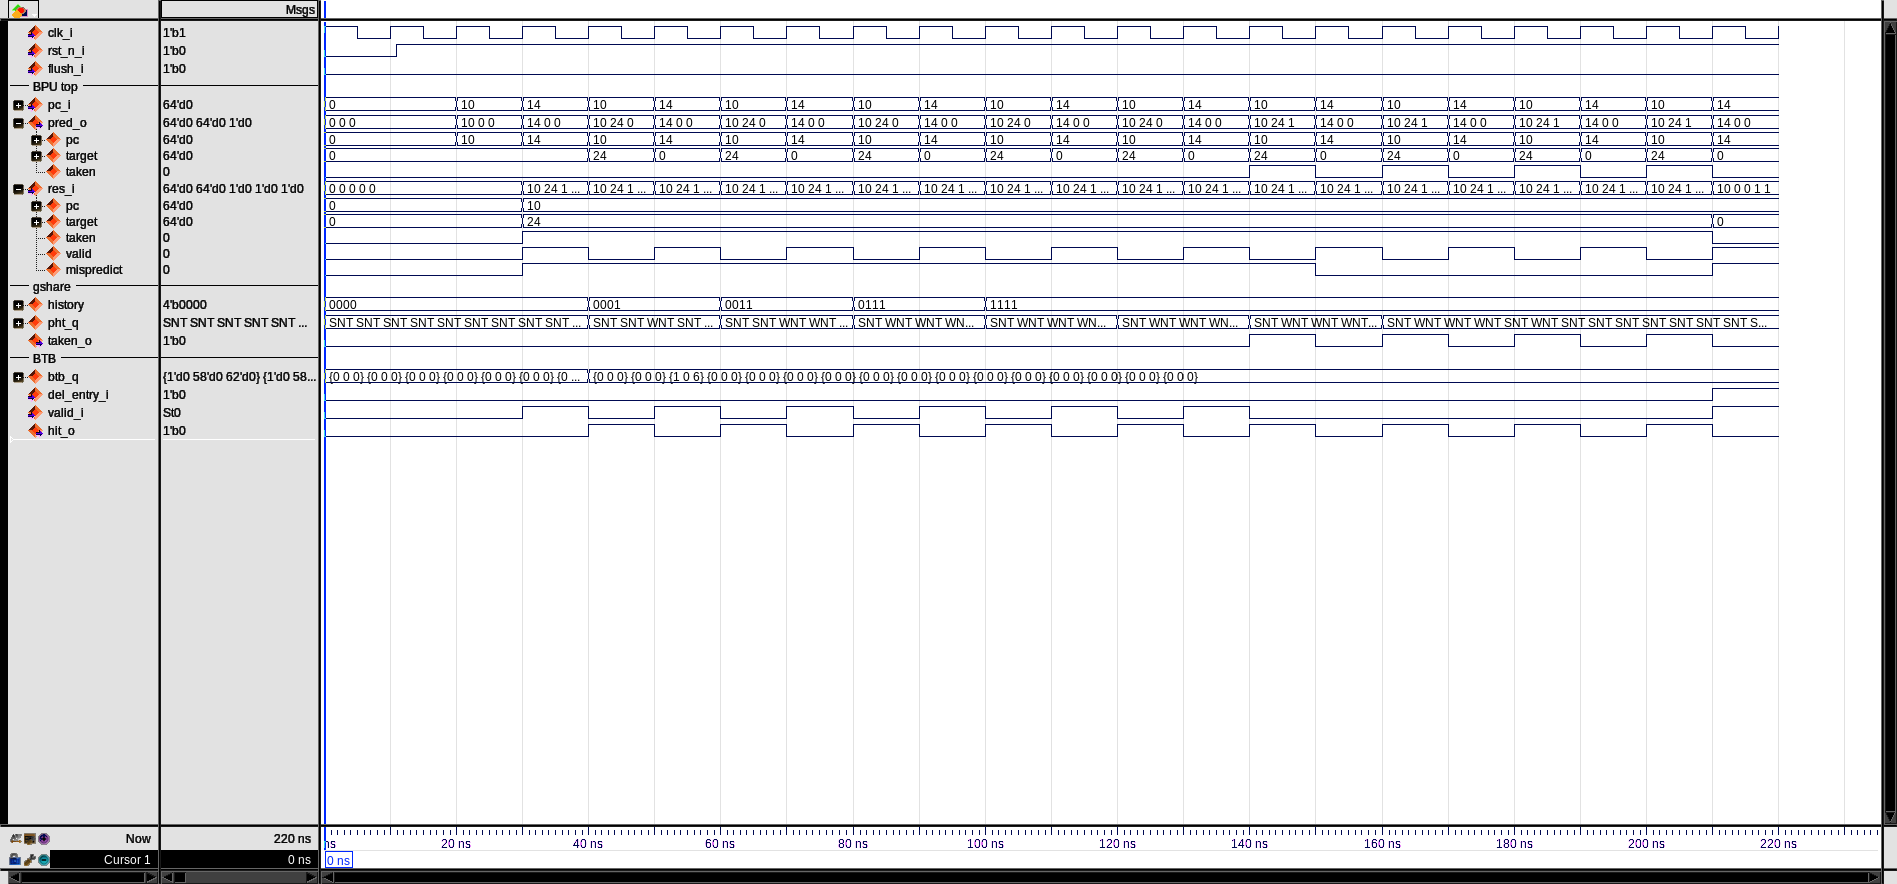
\includegraphics[width=\textheight]{img/bpu_loop01_conv.png}
  \caption{Single loop simulation}
  \label{fig:bpu_loop01_conv}
\end{sidewaysfigure}
Suppose that the instruction testing the loop condition is at address 10 and the beginning of the loop body (i.e.\ the target of the branch instruction) is at address 24. \Cref{fig:bpu_loop01_conv} shows the simulation waveforms for this test case, with the predictions contained in the \texttt{pred\_o} signal, occurring each time the \ac{PC} 10 is read from the address file, and the resolutions read into \texttt{res\_i} every time the \texttt{valid} signal is asserted.

Here, the initialization of the predictor structures can be clearly noted. Given that the history register is initialized to zero and the loop branch is always taken at first, the gshare predictor will initially update 2-bit counters which do not correspond to the actual branch history, until the \ac{BHT} is filled with ones (4 iterations, for the 4-bit register). Then the \ac{PHT} index will remain the same and so the same 2-bit counter is incremented from the initial strongly not taken state to the weakly taken state when it finally starts predicting correctly (2 iterations).

At the seventh iteration of the loop, the branch is predicted correctly as taken (the \texttt{mispredict} signal is deasserted) and this situation lasts until the the loop condition is tested false at the last iteration, leading to a new misprediction. 

Meanwhile, the \ac{BTB} is updated with the correct target at the first iteration, from which it gets a hit each following time.

This \emph{warm-up} of the predictor is intrinsic of its design and cannot be avoided, but anyway \cref{fig:bpu_loop01_conv} demonstrates the correct and expected behavior of the \ac{BPU}.

\subsubsection{Nested loops}
Next, the case of two nested loops was tested, as in the following code:
\begin{lstlisting}[language=C]
  for (int i = 0; i < 20; i++)
  {
    for (int j = 0; j < 3; j++)
    {
      /* loop body */
    }
  }
\end{lstlisting}
This example, actually taken from \cite{mcfarling93}, is intended to demonstrate that the gshare predictor, after the warm-up, can correctly identify taken branches in nested loops, where the outer loop is repeated many times.

\begin{sidewaysfigure}[p]
  \centering
  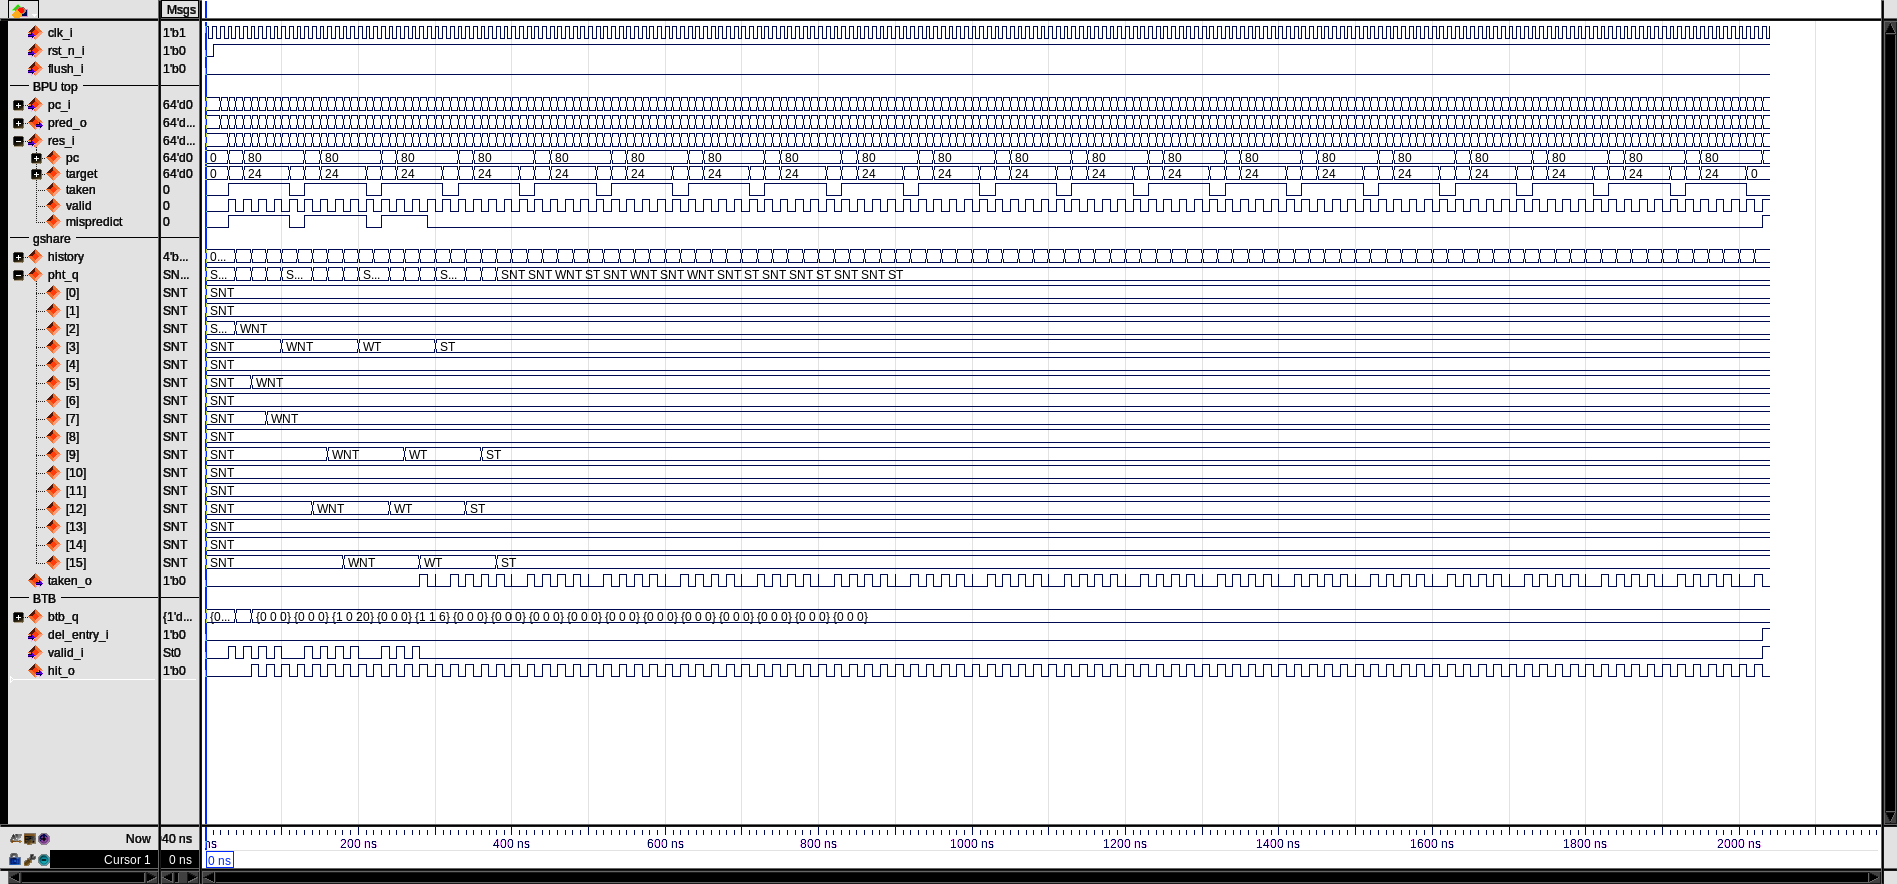
\includegraphics[width=\textheight]{img/bpu_loop02_conv.png}
  \caption{Nested loops simulation}
  \label{fig:bpu_loop02_conv}
\end{sidewaysfigure}
\Cref{fig:bpu_loop02_conv} shows the simulation results for this case, where the address of the condition instruction of the outer loop is 10, the one of the inner loop (i.e.\ the target of the outer loop) is 80 and the body of the inner loop starts at address 24. 

At the beginning, the gshare continuously mispredicts the outer loop and the first iterations of the inner loop, due to the initialization of the \ac{PHT} as mentioned in the previous case, but then after the warm-up it goes on to predict correctly both loops, until the exit of the outer loop. In particular, the steady state situation is shown in \cref{tab:nested}, where each combination of address and history univocally determines the prediction outcome.
\begin{table}[hbt]
  \centering
  \begin{tabular}{lllll}
    \toprule
    \textbf{Value} & \textbf{Condition} & \textbf{\ac{PC}} & \textbf{History} & \textbf{Prediction} \\ \midrule
    \texttt{j = 0} & \texttt{j < 3}   & 80  & 1101  & Taken     \\ \midrule
    \texttt{j = 1} & \texttt{j < 3}   & 80  & 1011  & Taken     \\ \midrule
    \texttt{j = 2} & \texttt{j < 3}   & 80  & 0111  & Taken     \\ \midrule
    \texttt{j = 3} & \texttt{j < 3}   & 80  & 1111  & Not taken \\ \midrule
    \texttt{i = n} & \texttt{i < 20}  & 10  & 1110  & Taken     \\
    \bottomrule
  \end{tabular}
  \caption{Nested loops steady state predictions}
  \label{tab:nested}
\end{table}

\subsection{Frontend}
The testbench designed for the whole frontend is composed of the following blocks that drive its inputs:
\begin{itemize}
  \item A \emph{\ac{PC} jumper} used to simulate exceptions and branches by modifying the sequential generation of addresses.
  \item A \emph{dummy instruction cache} which responds to memory access requests by simulating both hits and misses, with random delays. The fictional data line it provides always contains the \ac{PC} that generated the request and $N$ instruction fields with the number from 1 to $N$ in order to track the movement of instructions.
  \item A \emph{dummy issue queue} that simply simulates a busy issue queue by introducing random delays on the \texttt{issue\_ready} signal.
\end{itemize}

Using this setup, the frontend was simulated in a number of scenarios corresponding to the different situations analyzed in \cref{sec:frontend_timings}, of which the most significant are described below.

\Cref{fig:fetch01_conv} shows the standard situation where subsequent instructions are selected among the same line, saved in the line register after the first memory access at startup (compare with \cref{fig:fetch01}).

\Cref{fig:fetch02_address_conv,fig:fetch02_miss_conv} show the situation of a cache not ready to receive the address or a cache miss respectively, as in \cref{fig:fetch02}. Note also the current states of the instruction cache interface \acs{FSM} that correspond to the timing diagrams of \cref{fig:cache02,fig:cache03}\footnote{These simulation waveforms show \texttt{WAIT\_ADDR} as the wrong old name for the \texttt{WAIT\_REQ} state.}.

\Cref{fig:fetch07_conv} shows a sequence of cache reads in a pipeline fashion, just as in \cref{fig:fetch07}. Note also how here there is a jump right after the boot address, which is correctly handled by the instruction cache interface.

\Cref{fig:fetch09_conv}, like \cref{fig:fetch09}, show the case when the instruction is selected among the line backup register, due to a jump back and forth to the same cache line.

Finally as an example, \cref{fig:fetch03_conv} shows the situation in which the issue queue is not ready during instruction selection (compare with \cref{fig:fetch03}).

\begin{sidewaysfigure}[p]
  \centering
  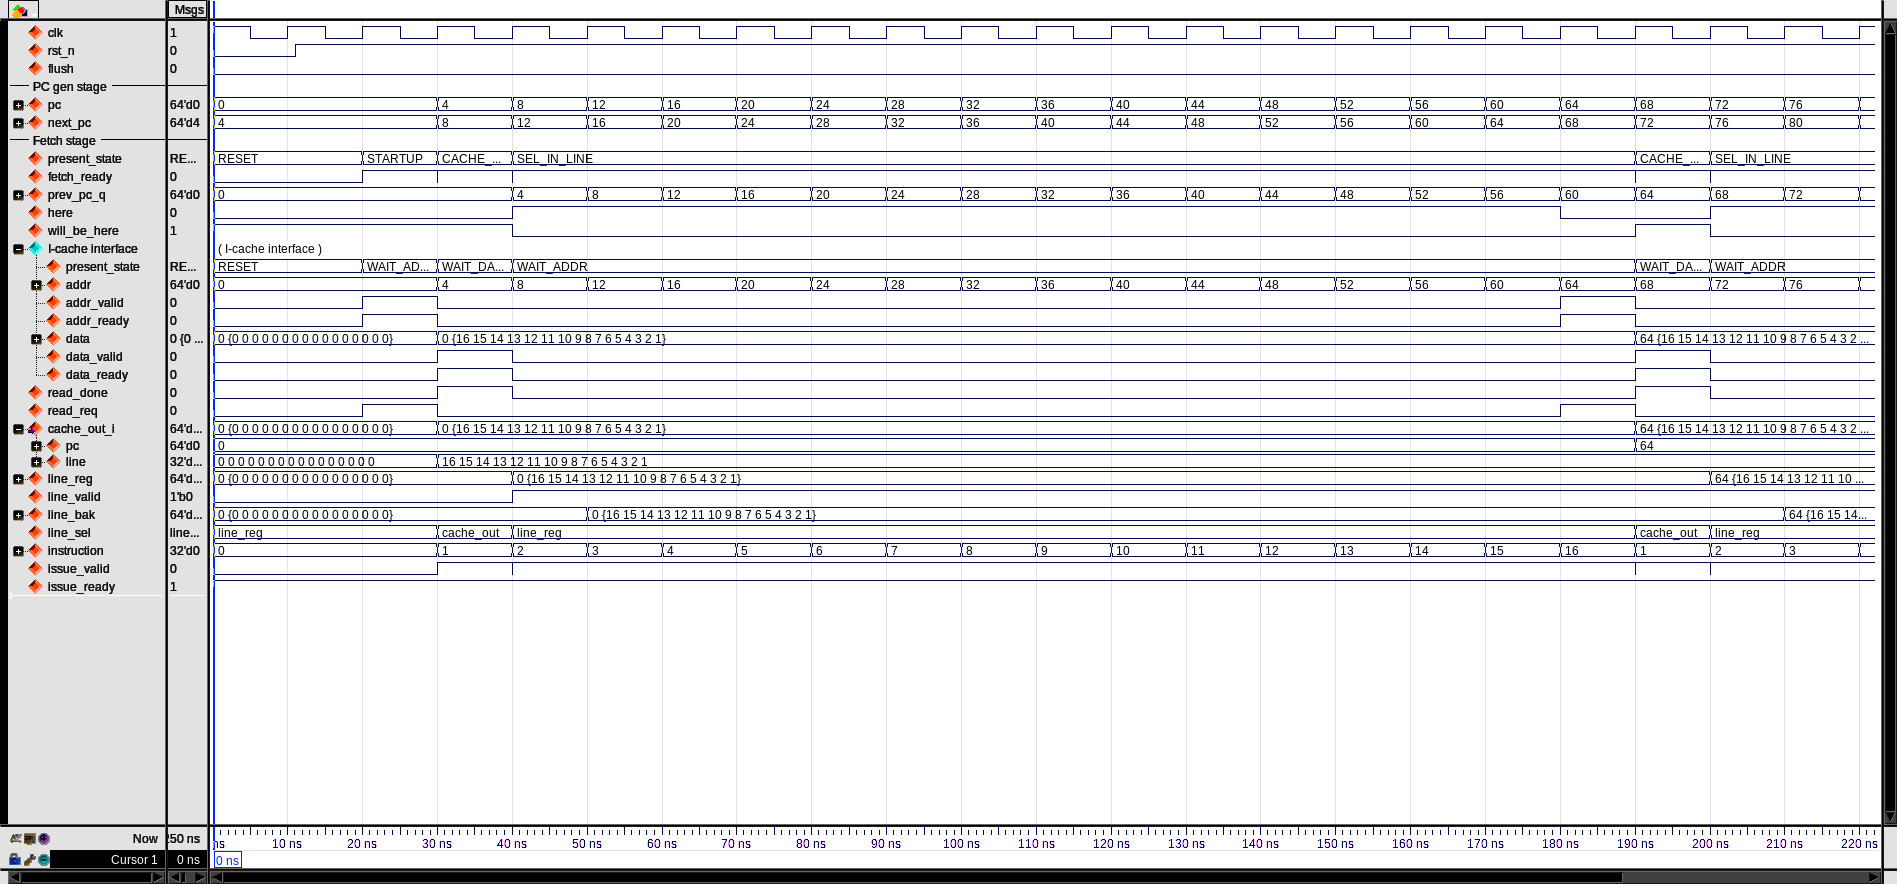
\includegraphics[width=\textheight]{img/fetch01_conv.png}
  \caption{Sequential reads from the same line}
  \label{fig:fetch01_conv}
\end{sidewaysfigure}
\begin{sidewaysfigure}[p]
  \centering
  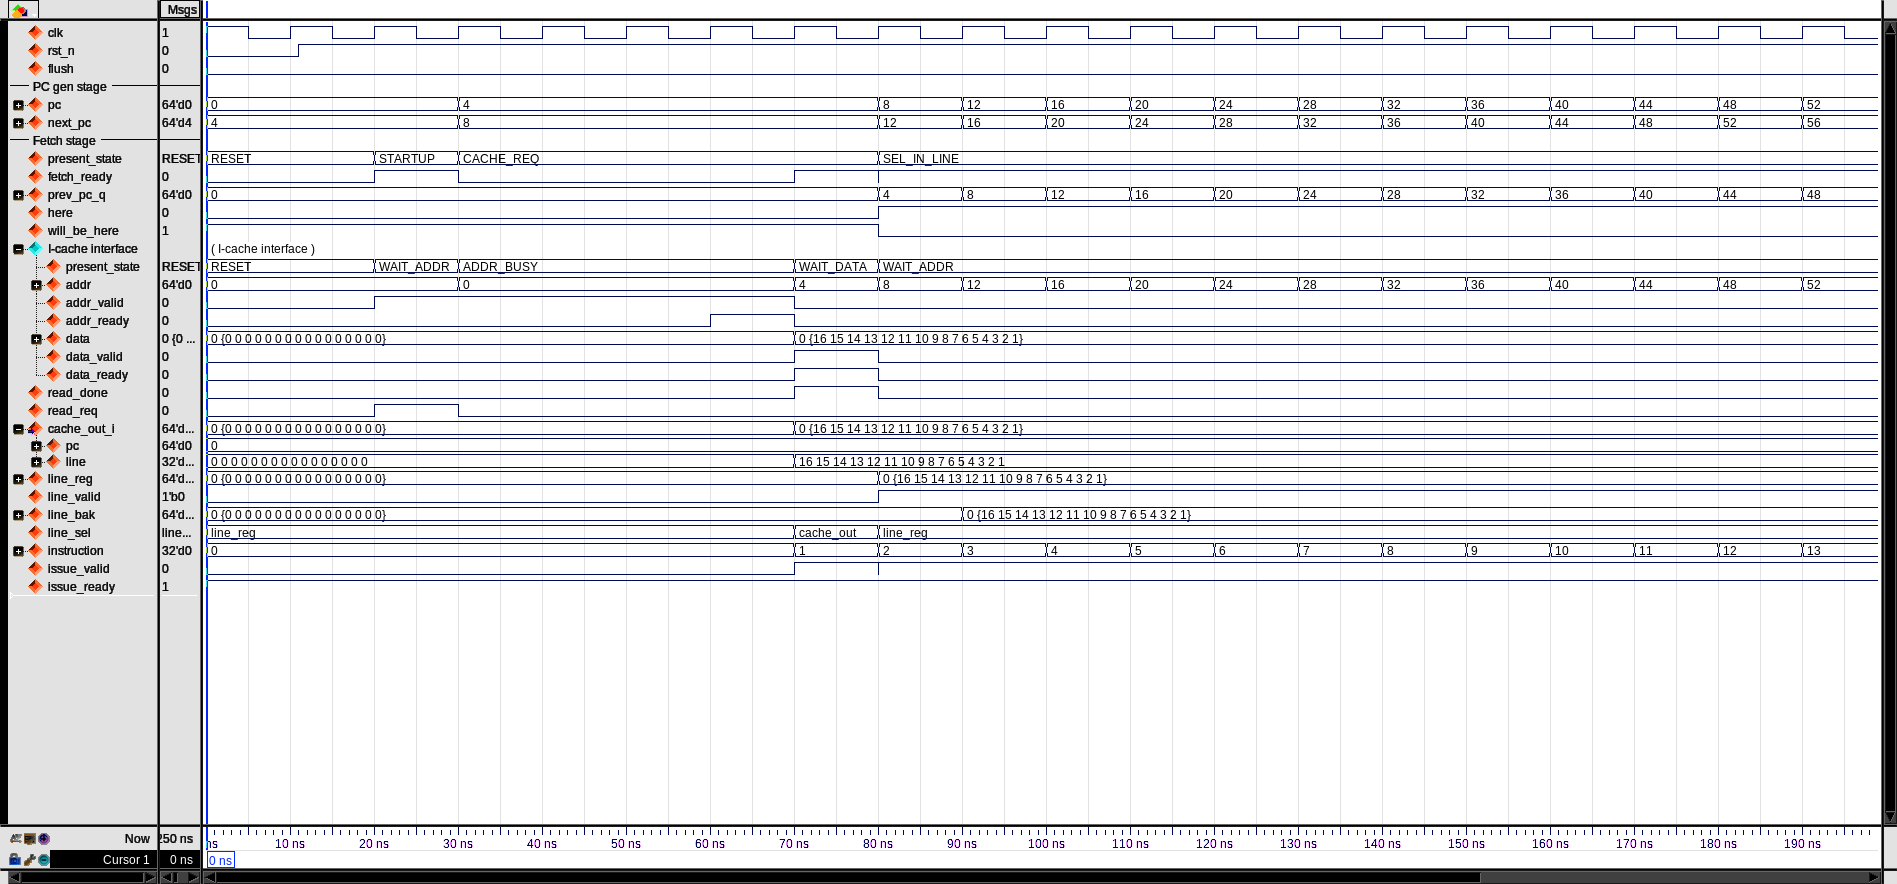
\includegraphics[width=\textheight]{img/fetch02_address_conv.png}
  \caption{Cache not ready on address}
  \label{fig:fetch02_address_conv}
\end{sidewaysfigure}
\begin{sidewaysfigure}[p]
  \centering
  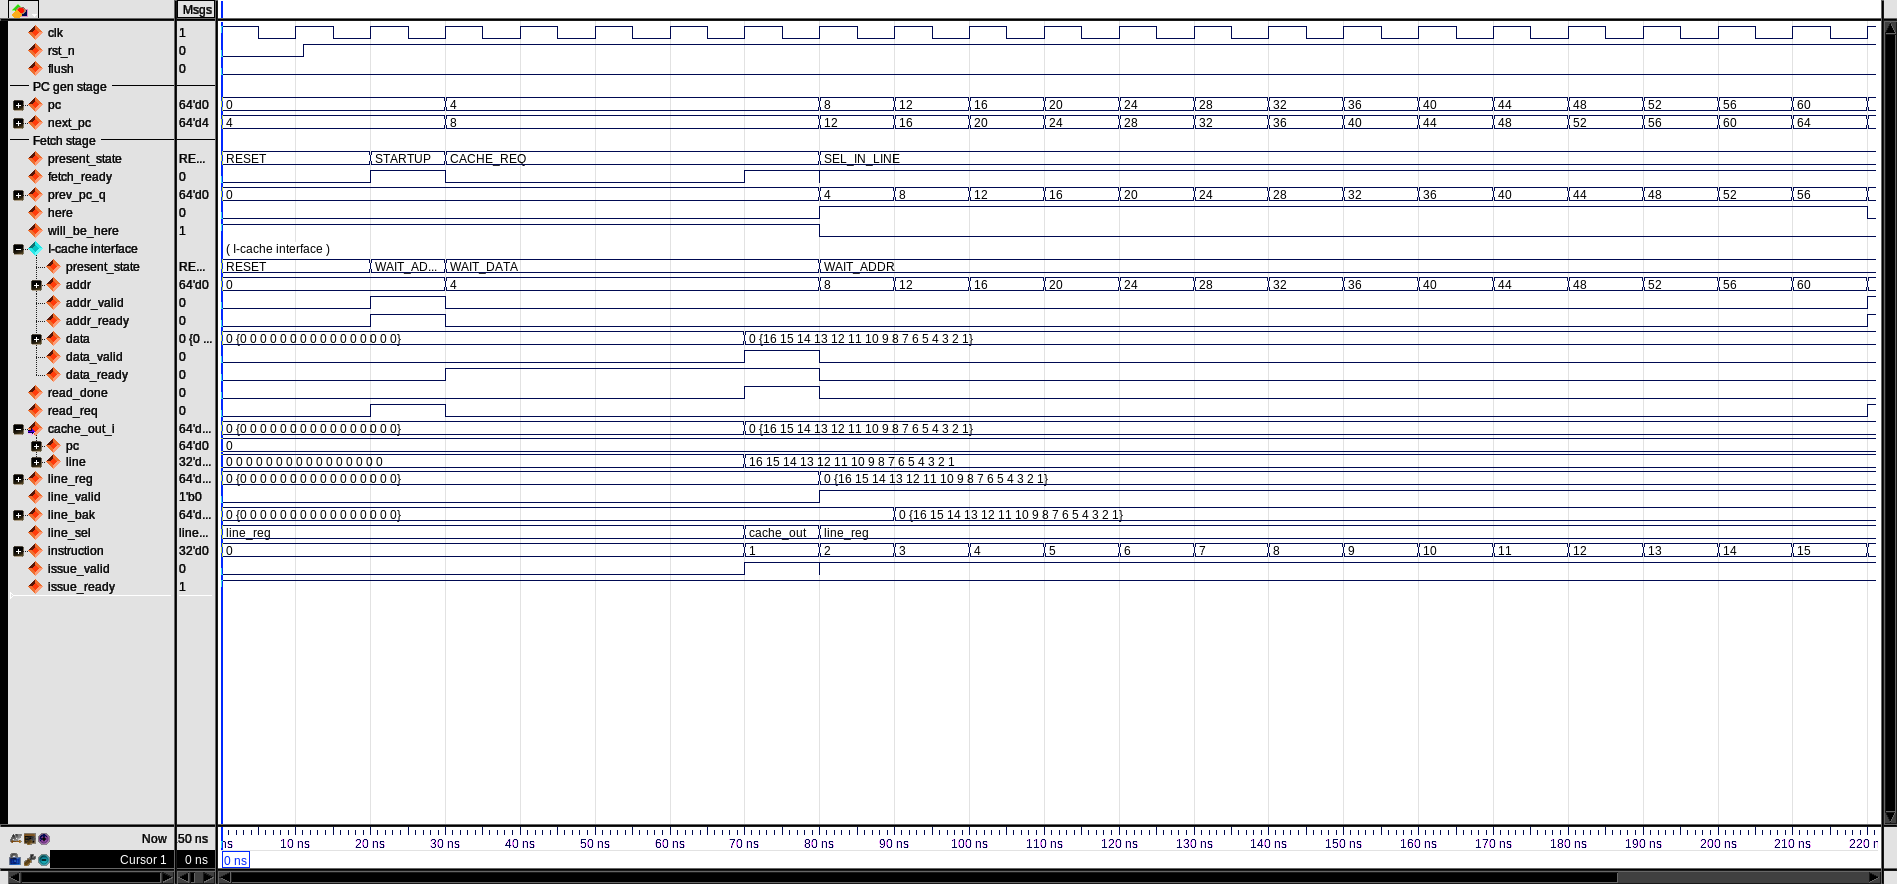
\includegraphics[width=\textheight]{img/fetch02_miss_conv.png}
  \caption{Cache miss}
  \label{fig:fetch02_miss_conv}
\end{sidewaysfigure}
\begin{sidewaysfigure}[p]
  \centering
  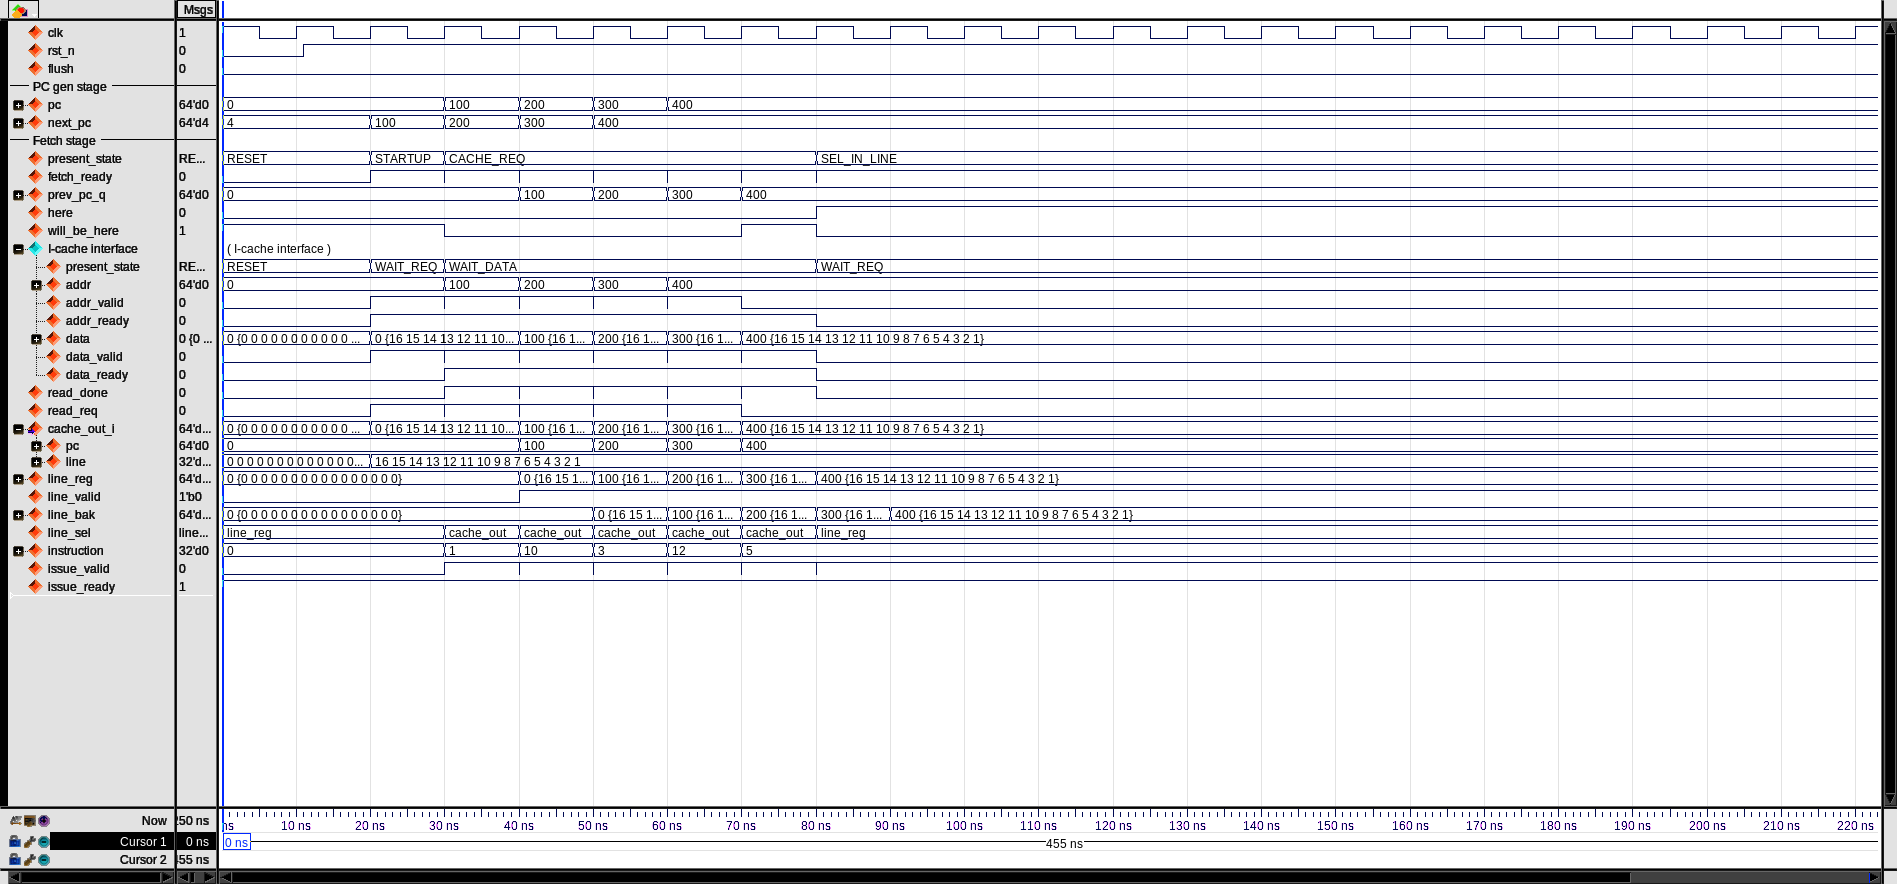
\includegraphics[width=\textheight]{img/fetch07_conv.png}
  \caption{Cache read pipeline}
  \label{fig:fetch07_conv}
\end{sidewaysfigure}
\begin{sidewaysfigure}[p]
  \centering
  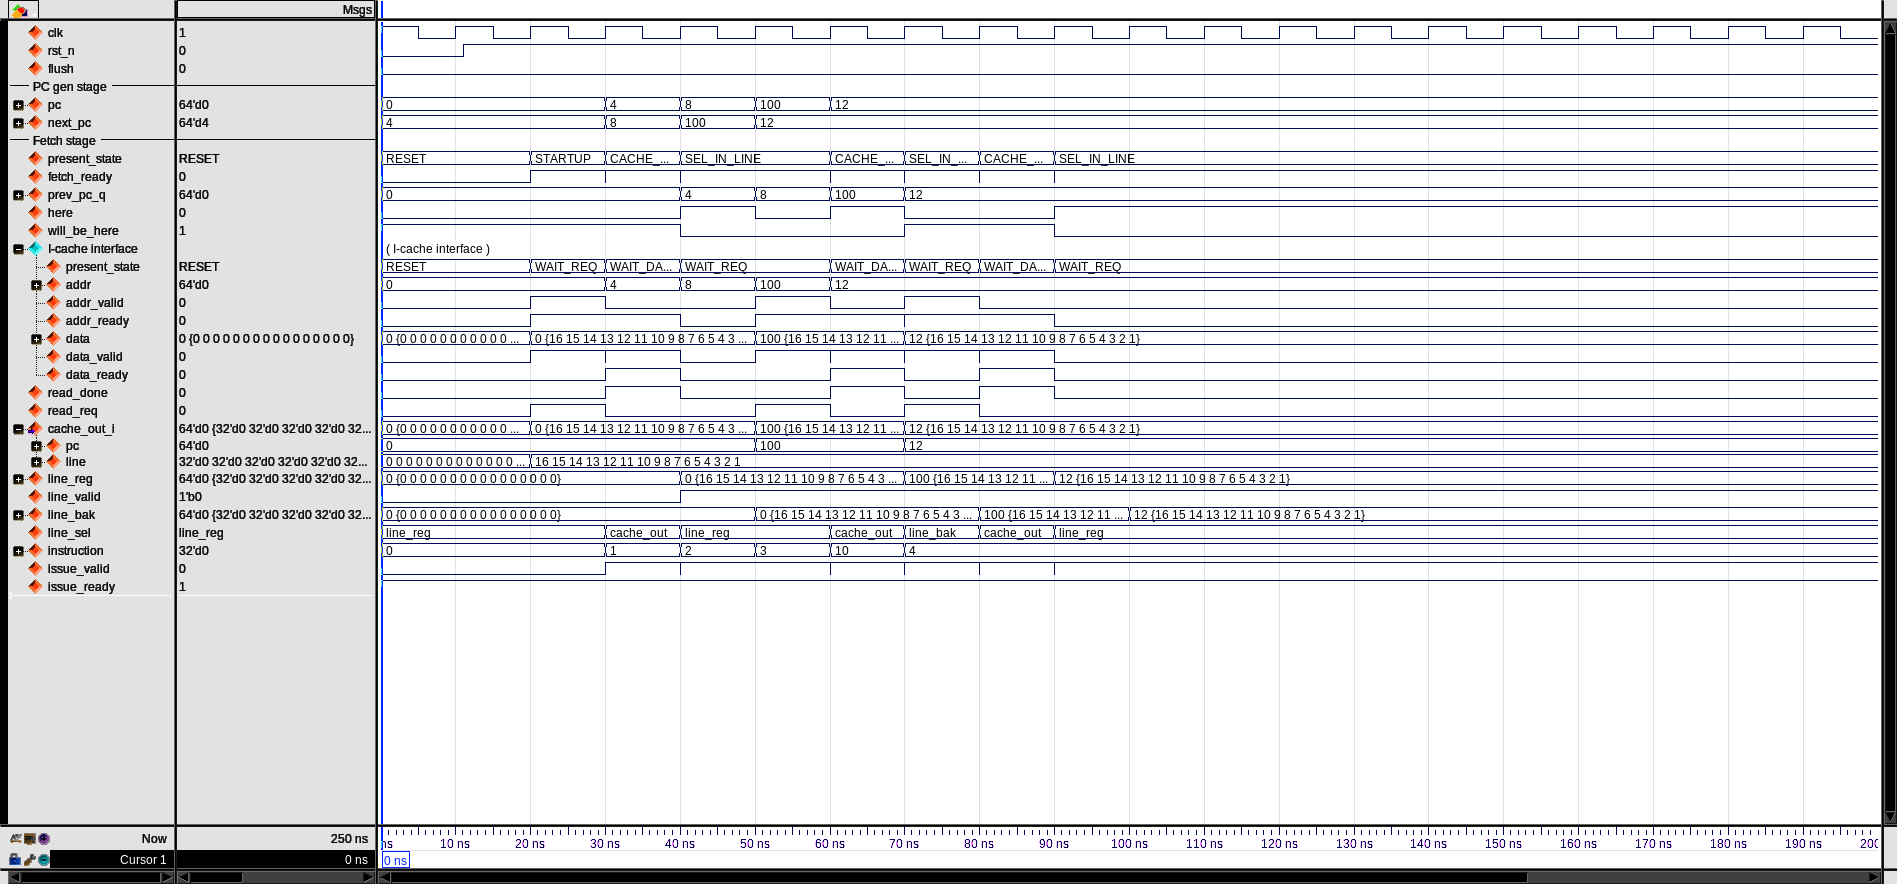
\includegraphics[width=\textheight]{img/fetch09_conv.png}
  \caption{Line backup register selection}
  \label{fig:fetch09_conv}
\end{sidewaysfigure}
\begin{sidewaysfigure}[p]
  \centering
  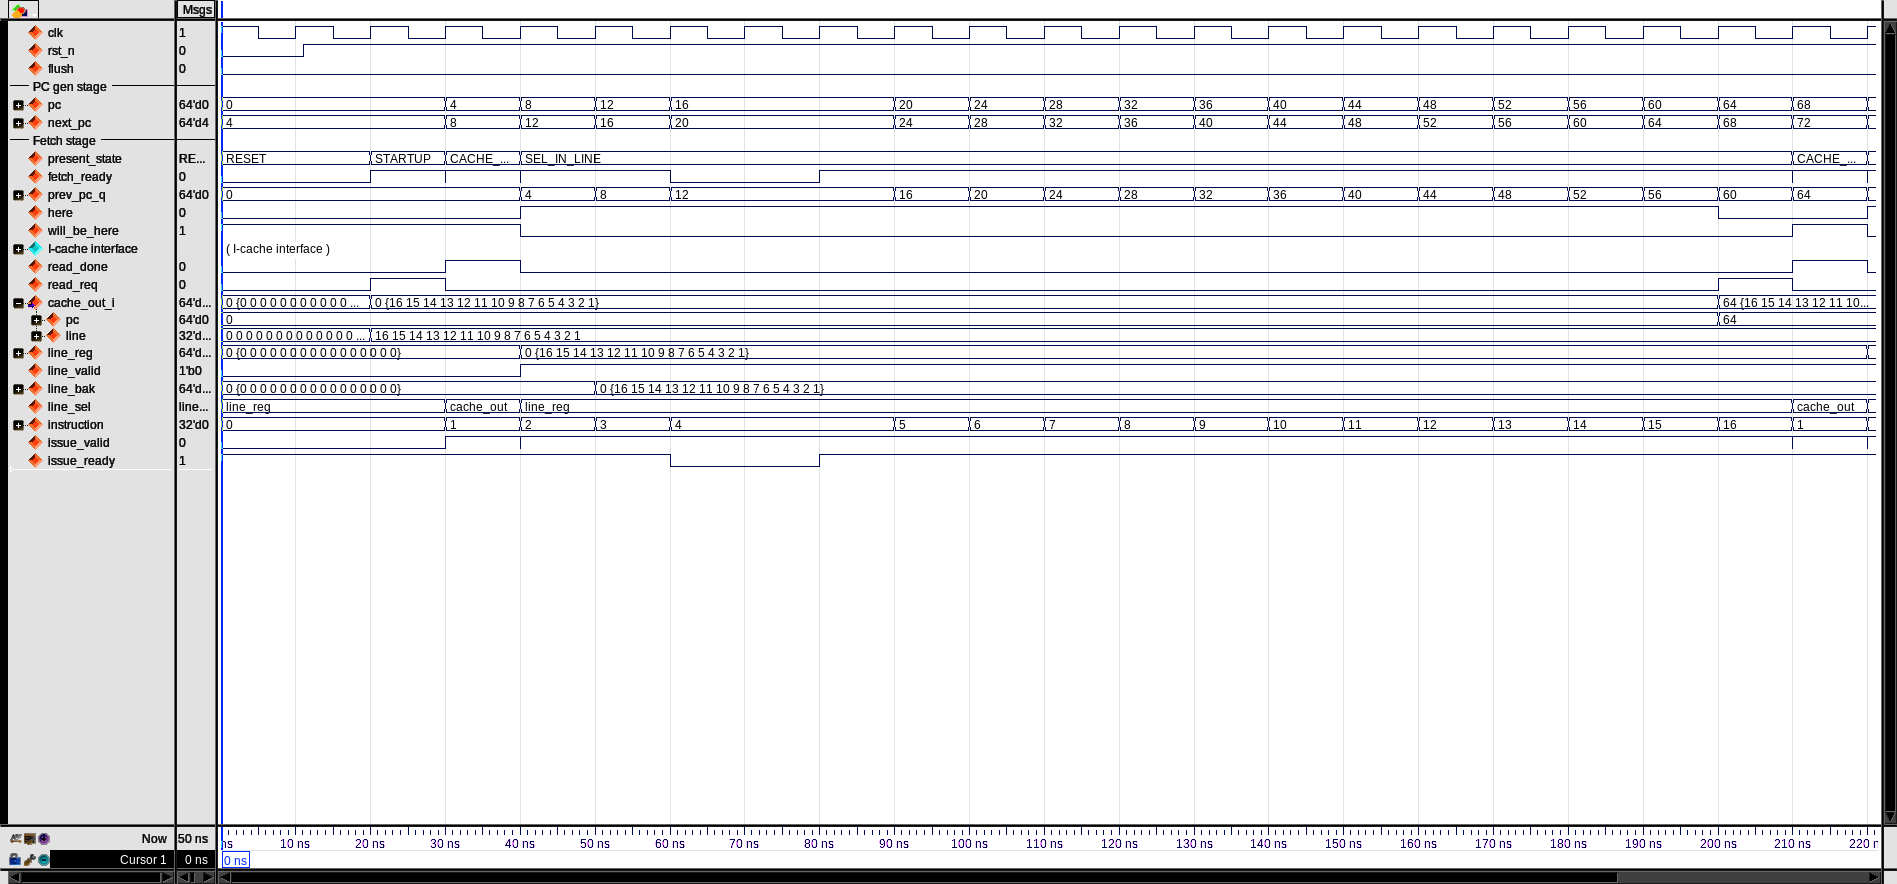
\includegraphics[width=\textheight]{img/fetch03_conv.png}
  \caption{Issue queue busy}
  \label{fig:fetch03_conv}
\end{sidewaysfigure}

\pagebreak
\section{\acs{BPU} benchmarking}
As mentioned before, the \ac{BPU} is one of the most configurable units in the design, where a number of parameters and design choices come into play. For this reason a software model of this module written in C has been developed, to allow for fast and simple exploration and benchmarking. The model implements the same functions as the hardware and reads an input text file in the form
\begin{center}
  \texttt{<BRANCH ADDRESS>}  \texttt{<OUTCOME>}
\end{center}
where the address is expressed in hexadecimal base and the outcome as 1 or 0 if the branch is taken or not.

After significant efforts spent to find a way to extract \emph{branch traces} (i.e.\ the list of branch instructions and their result) from a compiled program, no feasible solution was found and so a decision was made to rely on the trace files provided by a laboratory exercise of the course \emph{Principles in Computer Architecture} held by Prof. Dean Tullsen of the University of California San Diego, available on GitHub\footnote{\url{https://github.com/prodromou87/CSE240A}}. These traces come from a series of benchmarks taken from the SPEC suite, listed in \cref{tab:benchmarks}.
\begin{table}[hbt]
  \centering
  \begin{tabular}{lll}
    \toprule
    \textbf{Name}   & \textbf{Type}    & \textbf{Branches}  \\ \midrule
    \texttt{fp\_1}  & Floating point   & \num{1546797}      \\ \midrule
    \texttt{fp\_2}  & Floating point   & \num{2422049}      \\ \midrule
    \texttt{int\_1} & Integer          & \num{3771697}      \\ \midrule
    \texttt{int\_2} & Integer          & \num{3755315}      \\ \midrule
    \texttt{mm\_1}  & Matrix multiply  & \num{3014850}      \\ \midrule
    \texttt{mm\_2}  & Matrix multiply  & \num{2563897}      \\
    \bottomrule
  \end{tabular}
  \caption{\acs{BPU} benchmarks}
  \label{tab:benchmarks}
\end{table}

Given that these trace files do not contain the target address associated with each branch instruction, the main limitation of the software model is that it does not account for mispredictions caused by the wrong target being stored in the \ac{BTB}. It takes into account, however, the case when a \ac{BTB} too small causes entries to be overwritten frequently, increasing the number of misses and thus mispredictions.

In the following sections, a series of tests is described to evaluate performance and other design metrics on the \ac{BPU}.

\subsection{Gshare}\label{sec:gshare_bench}
For what concerns the gshare predictor, three main parameters can be analyzed:
\begin{itemize}
  \item The length of the history register, which determines the number of 2-bit counters in the \ac{PHT}.
  \item The initial value of those counters, which determines the first predictions for each index.
  \item The presence or not of the valid bit, along with each counter.
\end{itemize}

\subsubsection{2-bit counters initialization}
In order to find the best initial value for the counters, each benchmark was run on two different history register lengths (8 and 16 bits) at each possible initialization, including the alternate version even index/weakly not taken odd index/weakly taken.
\begin{table}[hbt]
  \centering
  \begin{tabular}{lllllll}
    \toprule
    \multirow{2}{*}{\textbf{Initial value}} & \multicolumn{6}{c}{\textbf{Benchmark}}                             \\
    \cmidrule{2-7}
                                   & \texttt{fp\_1}               & \texttt{fp\_2}                & \texttt{int\_1}               & \texttt{int\_2}               & \texttt{mm\_1}                & \texttt{mm\_2}                \\
    \midrule
    SNT                            & 98.35\%                      & 88.62\%                       & 69.09\%                       & \cellcolor{cell_blue}98.75\%  & \cellcolor{cell_blue}77.50\%  & 82.37\%                       \\
    WNT                            & 98.36\%                      & 88.55\%                       & 69.09\%                       & 98.75\%                       & 77.50\%                       & \cellcolor{cell_blue}82.37\%  \\
    WT                             & 98.36\%                      & \cellcolor{cell_blue}89.90\%  & \cellcolor{cell_blue}69.09\%  & 98.74\%                       & 77.49\%                       & 82.37\%                       \\
    ST                             & 98.27\%                      & 89.90\%                       & 69.09\%                       & 98.74\%                       & 77.50\%                       & 82.37\%                       \\
    even/WNT, odd/WT               & \cellcolor{cell_blue}98.36\% & 88.65\%                       & 69.09\%                       & 98.74\%                       & 77.50\%                       & 82.37\%                       \\
    \bottomrule
  \end{tabular}
  \caption{Gshare accuracy on different initializations (8-bit history register)}
  \label{tab:init8}
\end{table}
\begin{table}[hbt]
  \centering
  \begin{tabular}{lllllll}
    \toprule
    \multirow{2}{*}{\textbf{Initial value}} & \multicolumn{6}{c}{\textbf{Benchmark}}                             \\
    \cmidrule{2-7}
                                   & \texttt{fp\_1}               & \texttt{fp\_2}                & \texttt{int\_1}               & \texttt{int\_2}               & \texttt{mm\_1}                & \texttt{mm\_2}                \\
    \midrule
    SNT                            & 99.15\%                      & 99.03\%                       & \cellcolor{cell_blue}89.24\% & 99.63\%                        & \cellcolor{cell_blue}96.05\%  & 92.28\%                       \\
    WNT                            & \cellcolor{cell_blue}99.17\% & 98.85\%                       & 88.26\%                      & \cellcolor{cell_blue}99.64\%   & 95.86\%                       & 92.83\%                       \\
    WT                             & 99.16\%                      & \cellcolor{cell_blue}99.04\%  & 89.11\%                      & 99.64\%                        & 95.88\%                       & \cellcolor{cell_blue}92.87\%  \\
    ST                             & 99.15\%                      & 99.04\%                       & 89.23\%                      & 99.61\%                        & 95.97\%                       & 92.39\%                       \\
    even/WNT, odd/WT               & 99.17\%                      & 99.04\%                       & 88.65\%                      & 99.64\%                        & 95.88\%                       & 92.84\%                       \\ 
    \bottomrule
  \end{tabular}
  \caption{Gshare accuracy on different initializations (16-bit history register)}
  \label{tab:init16}
\end{table}

\pagebreak
The results are summarized in \cref{tab:init8,tab:init16} for 8-bit and 16-bit history registers respectively, where blue cells represent the best accuracy achieved for each benchmark. It is clear that there is no single best initialization value for the 2-bit counters, but it depends heavily on both the benchmark and the history length. Even the most complex initialization to be performed in hardware, which is the alternate one, results the best only in a single case. In any case, there is not much of a difference among the various initial values, so the conclusion is to choose the simplest one, namely the strongly not taken state (i.e.\ 2-bit counters at zero).

\subsubsection{Valid bit}
From the results of the previous analysis, it is obvious that the valid bit serves no purpose whatsoever in this design. A valid bit would be used to indicate that the indexed counter has been used before and so the prediction is valid. By initializing the 2-bit counters to zero, however, the first (and second) time they are read, they are always going to predict not taken, exactly like the case with the valid bit. In the end, this bit would only increase by 50\% the total \ac{PHT} size, thus literally wasting a significant amount of area.

\subsubsection{History register length}
In order to find the best trade-off between the predictor accuracy and the size of the \ac{PHT}, all the benchmarks were run at increasingly longer history length.
\begin{figure}[hbt]
  \centering
%   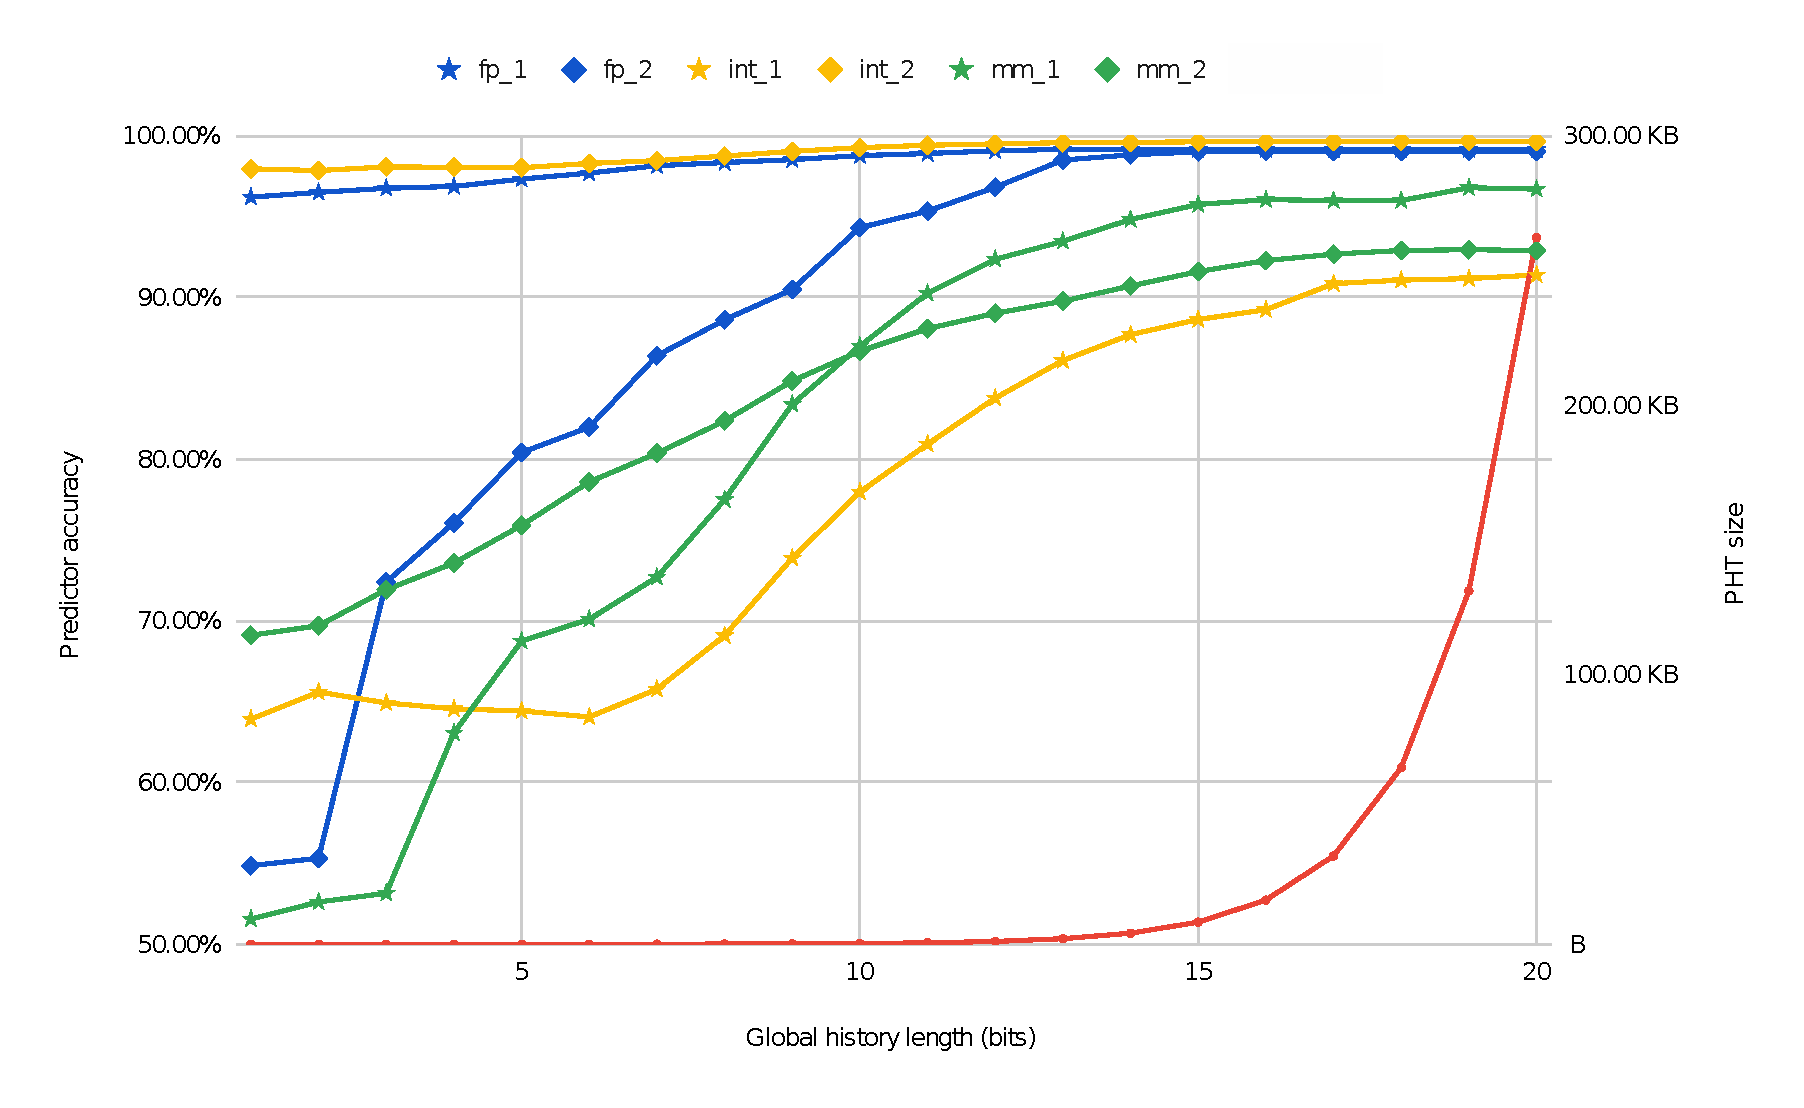
\includegraphics[width=\textwidth]{img/pht_size.pdf}
    \begin{tikzpicture}
      \pgfplotsset{
        width=0.75\textwidth,
        height=0.5\textwidth,  
        scale only axis,
        xmin=1, xmax=20,
      }
      \begin{axis}[
        ymin=50, ymax=100,
        yticklabel={$\pgfmathprintnumber{\tick}$\%},
        axis y line*=left,
        xlabel={Global history length (bits)},
        ylabel={Predictor accuracy},
        xtick={1,5,10,15,20},
        ytick={50,60,70,80,90,100}
      ]
      
        \addplot[color=plot_blue,mark=triangle*,very thick]
          table [x={hLen},y={fp_1}] {data/hlen.dat}; \label{fp_1}
        \addplot[color=plot_blue,mark=diamond*,very thick]
          table [x={hLen},y={fp_2}] {data/hlen.dat}; \label{fp_2}
        \addplot[color=plot_yellow,mark=triangle*,very thick]
          table [x={hLen},y={int_1}] {data/hlen.dat}; \label{int_1}
        \addplot[color=plot_yellow,mark=diamond*,very thick]
          table [x={hLen},y={int_2}] {data/hlen.dat}; \label{int_2}
        \addplot[color=plot_green,mark=triangle*,very thick]
          table [x={hLen},y={mm_1}] {data/hlen.dat}; \label{mm_1}
        \addplot[color=plot_green,mark=diamond*,very thick]
          table [x={hLen},y={mm_2}] {data/hlen.dat}; \label{mm_2}
      \end{axis}

      \begin{axis}[
        ymin=0, ymax=300,
        axis y line*=right,
        axis x line=none,
        legend style={
          at={(0.5,1.2)},
          anchor=north,
          legend columns=7
        },
        ylabel={PHT size (KB)},
        ytick={50,100,150,200,250,300},
      ]
      
        \addlegendimage{/pgfplots/refstyle=fp_1}\addlegendentry{\texttt{fp\_1}}
        \addlegendimage{/pgfplots/refstyle=fp_2}\addlegendentry{\texttt{fp\_2}}
        \addlegendimage{/pgfplots/refstyle=int_1}\addlegendentry{\texttt{int\_1}}
        \addlegendimage{/pgfplots/refstyle=int_2}\addlegendentry{\texttt{int\_2}}
        \addlegendimage{/pgfplots/refstyle=mm_1}\addlegendentry{\texttt{mm\_1}}
        \addlegendimage{/pgfplots/refstyle=mm_2}\addlegendentry{\texttt{mm\_2}}

        \addplot[color=plot_red,mark=triangle*,very thick]
          table [x={hLen},y={phtSize}] {data/hlen.dat};
          \addlegendentry{PHT size}
      \end{axis}
    \end{tikzpicture}
  \caption{History register length versus predictor accuracy}
  \label{fig:pht_size}
\end{figure}

From the plot of \cref{fig:pht_size}, the majority of the benchmarks saturate at their best accuracy value in the range between 13 and 20 bits, with only \texttt{int\_1} and \texttt{mm\_1} being the exceptions that continue to get better results the longer the history. 

Given the exponential relation between the history register length and the area of the \ac{PHT}, this range of lengths corresponds to table sizes going from \SI{2}{KB} to \SI{200}{KB}. For this reason, the final value must be chosen by keeping in mind a clear area budget for the final implementation. Having said that, a history length of 16 bits, corresponding to around \SI{16}{KB} of \ac{PHT}, seems like a reasonable compromise for which benchmark results are no more than 2\% worse than the best.

\subsection{\acs{BTB}}
The \ac{BTB} on its own does not contribute to improving the overall prediction accuracy, which only comes from the gshare predictor itself, but instead removes the target computation latency from branch instructions. Thus, its presence can only lower the prediction accuracy with respect to the baseline of the gshare alone, because additional mispredictions are inserted due to \ac{BTB} misses, which occur when the \ac{BTB} does not have a valid entry for the selected address. Moreover, mispredictions take place even when the stored target is then discovered as incorrect, but as mentioned above the available branch traces do not contain the correct target, so the software model does not take this kind of mispredictions into account, which contribute only in small part anyway.
\begin{figure}[hbt]
  \centering
  % 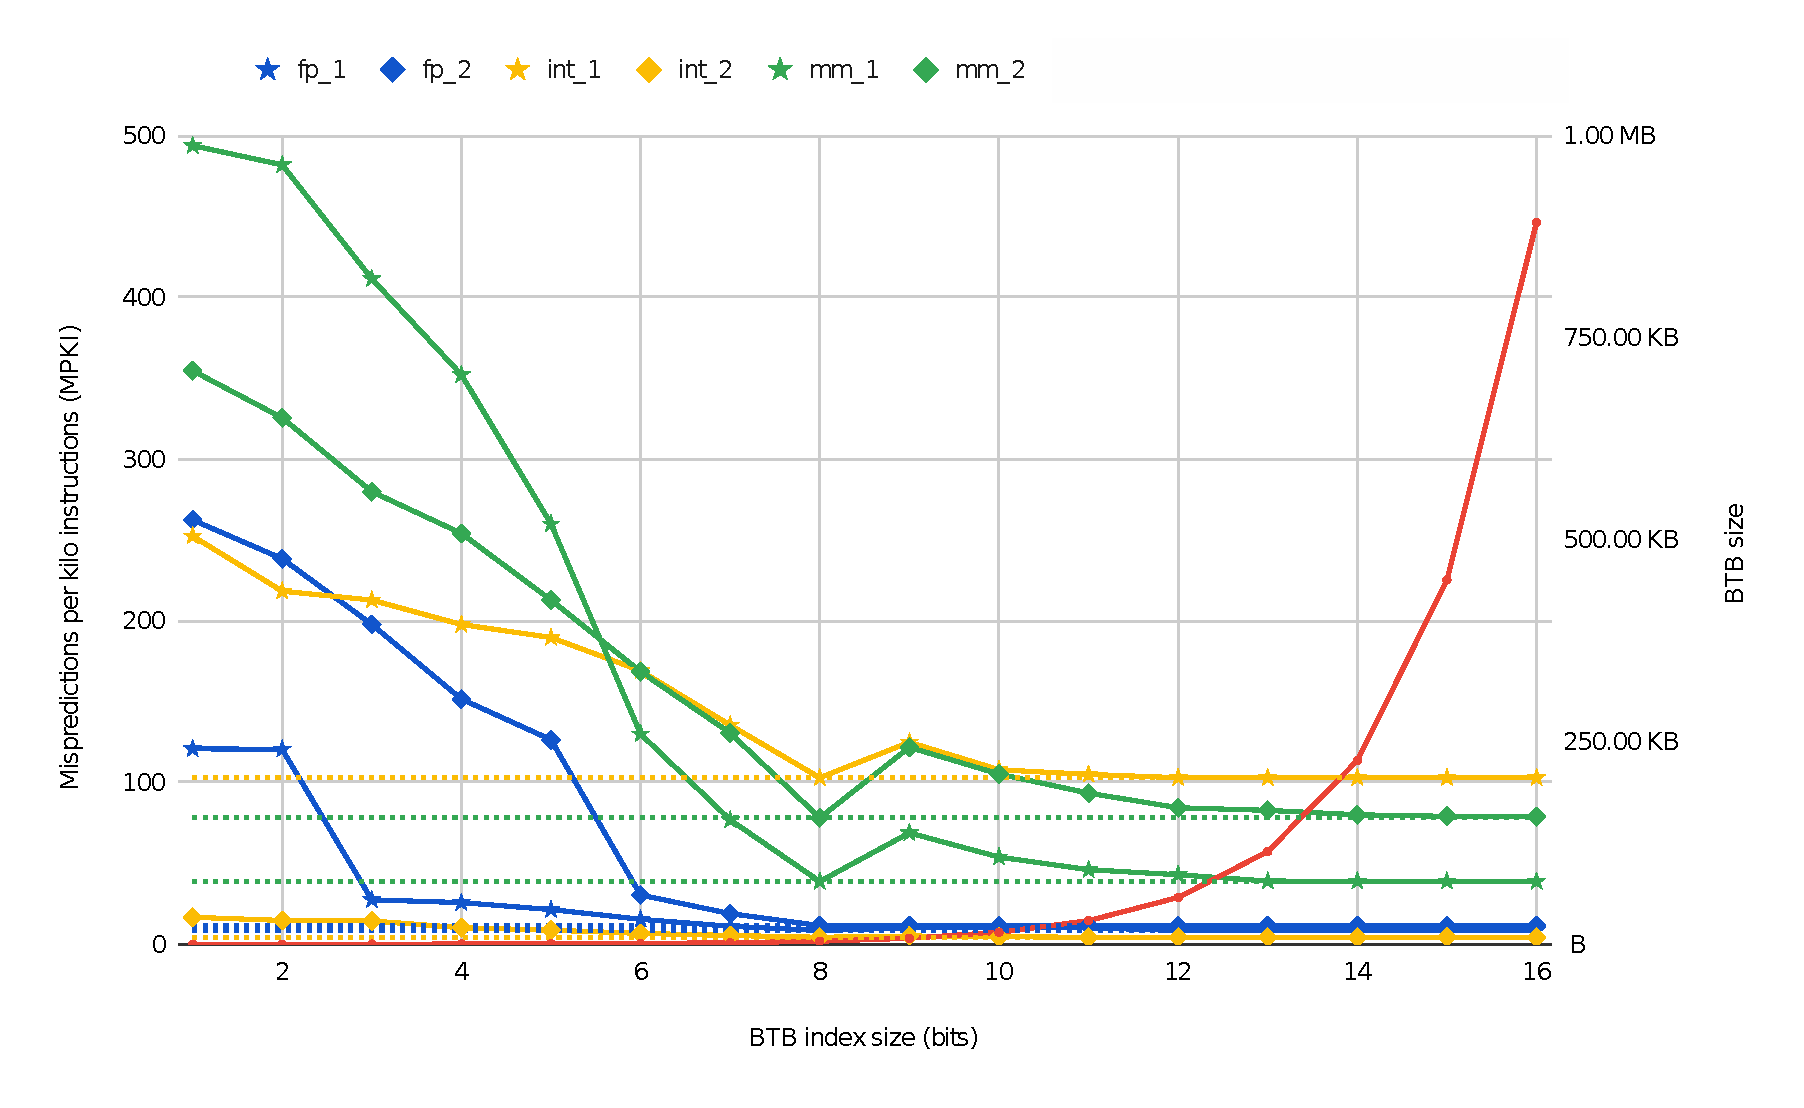
\includegraphics[width=\textwidth]{img/btb_size.pdf}
  \begin{tikzpicture}
    \pgfplotsset{
      width=0.75\textwidth,
      height=0.5\textwidth,  
      scale only axis,
      xmin=1, xmax=16,
    }
    \begin{axis}[
      ymin=0, ymax=500,
      axis y line*=left,
      xlabel={BTB index length (bits)},
      ylabel={Mispredictions per kilo instructions (MPKI)},
      xtick={2,4,6,8,10,12,14,16},
      ytick={0,100,200,300,400,500}
    ]
    
      \addplot[color=plot_blue,mark=triangle*,very thick]
        table [x={btbBits},y={fp_1}] {data/btb.dat}; \label{fp_1}
      \addplot[color=plot_blue,dashed]
        coordinates {(1, 8.478) (16, 8.478)};
      \addplot[color=plot_blue,mark=diamond*,very thick]
        table [x={btbBits},y={fp_2}] {data/btb.dat}; \label{fp_2}
      \addplot[color=plot_blue,dashed]
        coordinates {(1, 11.548) (16, 11.548)};
      \addplot[color=plot_yellow,mark=triangle*,very thick]
        table [x={btbBits},y={int_1}] {data/btb.dat}; \label{int_1}
      \addplot[color=plot_yellow,dashed]
        coordinates {(1, 102.991) (16, 102.991)};
      \addplot[color=plot_yellow,mark=diamond*,very thick]
        table [x={btbBits},y={int_2}] {data/btb.dat}; \label{int_2}
      \addplot[color=plot_yellow,dashed]
        coordinates {(1, 4.301) (16, 4.301)};
      \addplot[color=plot_green,mark=triangle*,very thick]
        table [x={btbBits},y={mm_1}] {data/btb.dat}; \label{mm_1}
      \addplot[color=plot_green,dashed]
        coordinates {(1, 38.844) (16, 38.844)};
      \addplot[color=plot_green,mark=diamond*,very thick]
        table [x={btbBits},y={mm_2}] {data/btb.dat}; \label{mm_2}
      \addplot[color=plot_green,dashed]
        coordinates {(1, 78.179) (16, 78.179)};
    \end{axis}

    \begin{axis}[
      ymin=0, ymax=1000,
      axis y line*=right,
      axis x line=none,
      legend style={
        at={(0.5,1.2)},
        anchor=north,
        legend columns=7
      },
      ylabel={PHT size (KB)},
      ytick={250,500,750,1000},
    ]
    
      \addlegendimage{/pgfplots/refstyle=fp_1}\addlegendentry{\texttt{fp\_1}}
      \addlegendimage{/pgfplots/refstyle=fp_2}\addlegendentry{\texttt{fp\_2}}
      \addlegendimage{/pgfplots/refstyle=int_1}\addlegendentry{\texttt{int\_1}}
      \addlegendimage{/pgfplots/refstyle=int_2}\addlegendentry{\texttt{int\_2}}
      \addlegendimage{/pgfplots/refstyle=mm_1}\addlegendentry{\texttt{mm\_1}}
      \addlegendimage{/pgfplots/refstyle=mm_2}\addlegendentry{\texttt{mm\_2}}

      \addplot[color=plot_red,mark=triangle*,very thick]
        table [x={btbBits},y={btbSize}] {data/btb.dat};
        \addlegendentry{BTB size}
    \end{axis}
  \end{tikzpicture}
  \caption{\acs{BTB} index size versus MPKI}
  \label{fig:btb_size}
\end{figure}

\Cref{fig:btb_size} shows the results of the benchmarks with varying length of the \ac{BTB} index expressed as the number of mispredictions per a thousand instructions (MPKI), where dashed lines represent the baseline without \ac{BTB} for each benchmark. Some programs, like \texttt{mm\_1} and \texttt{mm\_2} suffer significantly with small \acs{BTB} and have unacceptably high misprediction rates, while other, notably \texttt{int\_2} seem almost unaffected by the presence of the \ac{BTB}. Anyway, around 10 or 12 bits for the \ac{BTB} index, i.e.\ in the range \SI{15}{KB} to \SI{60}{KB}, most of the benchmark have reached a MPKI very close to the baseline. Going past these values does not seem to offer a significant improvement and thus becomes unadvisable, regardless of the area constraints.

\pagebreak
\section{Synthesis}
Synthesis has been carried out using Synopsys Design Compiler on the UMC \SI{65}{nm} low leakage (L65LL) technology library. In order to get reproducible results, scripting was heavily used to input commands to the tool and some notable parameters and settings used in the process are listed below:
\begin{itemize}
  \item Top down compilation, to allow optimizations beyond module boundaries, even if this means potentially longer compile times and higher memory usage, as stated in \cite[p.8-6]{dc}.
  \item Ideal clock definition (\texttt{set\_ideal\_network} and \texttt{set\_dont\_touch\_network}) in order to avoid optimizations on the clock tree, which has to be defined in later place and route stages, and remove warnings about its high fanout.
  \item Clock uncertainty (skew) \SI{0.07}{ns}
  \item Maximum input and output delay \SI{0.5}{ns}
  \item Output load of a buffer on all ports (\texttt{BUFM10R}, \SI{2.1}{\femto\farad})
  \item DC Expert compilation (\texttt{compile} command)
\end{itemize}

\subsection{\acs{BPU}}
The \ac{BPU} was synthesized in different configurations of history register length and \ac{BTB} size, in order to evaluate the effect of these parameters variations on the design metrics. In particular, from the considerations and the results obtained during benchmarking, the aim was to vary the history length between 2 and 16 bits and the \ac{BTB} index length from 2 to 12 bits. However, when trying to go past 12 bits of history and 10 for the \ac{BTB} index, Design Compiler could not sustain the exponential size of the register files and gave up with errors about exceeding the maximum loop iterations possible, nonetheless the results are still significant. Even then, the syntheses, executed with a batch script, took several days to complete.

\subsubsection{Area}
The total area of the \ac{BPU} depends almost exclusively on the size of the gshare \ac{PHT} and the \ac{BTB}, which are determined by the history length and the \ac{BTB} index bits. More specifically, given that each entry of the \ac{BTB} easily contains more than 100 bits compared to the 2 bits of a \ac{PHT} entry, the effect of the \ac{BTB} size will weigh 100 times more than the history length on the overall result. In other words, the length of the history register matters only with small \acp{BTB}, while it becomes negligible alongside large buffers.

\begin{figure}[hbt]
  \centering
  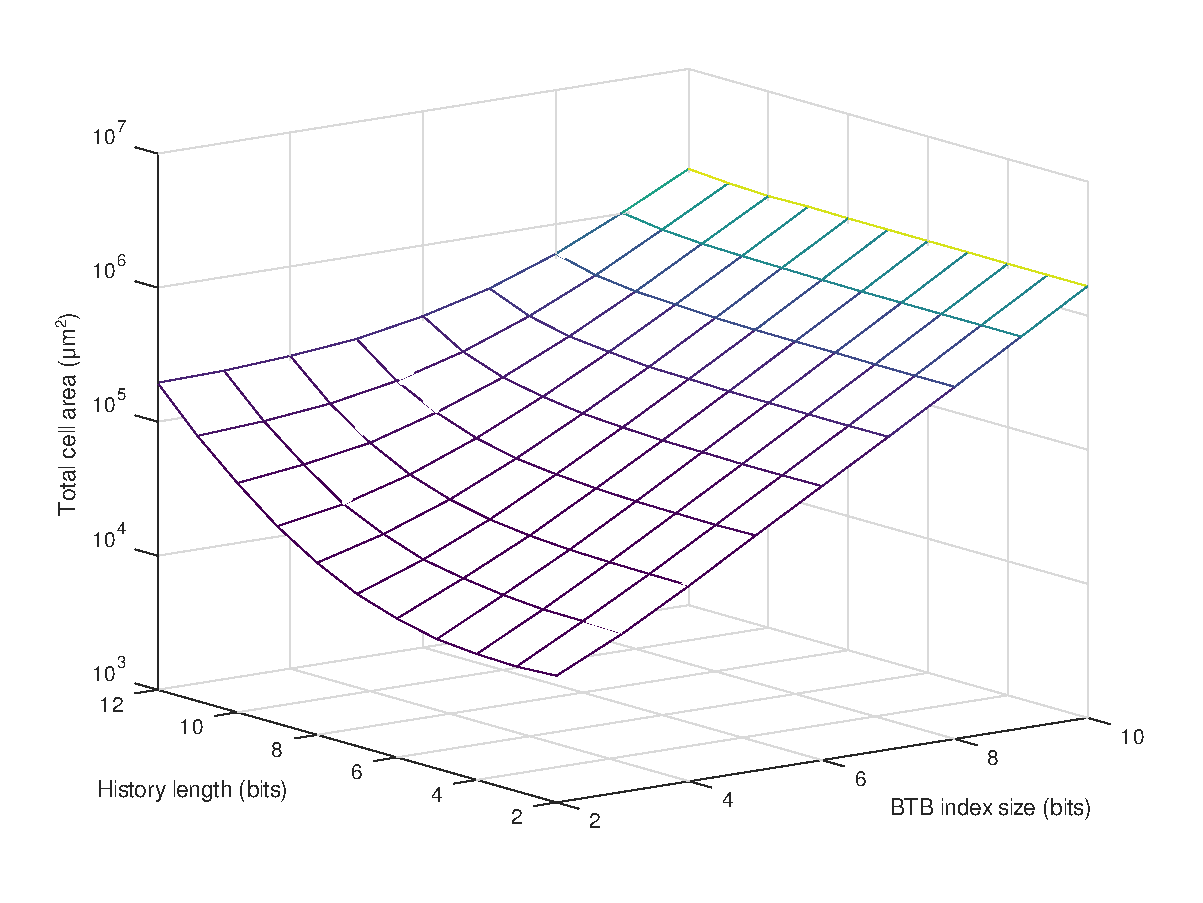
\includegraphics[width=\textwidth]{img/bpu_area.pdf}
  \caption{Total \acs{BPU} area versus history length and \ac{BTB} size}
  \label{fig:bpu_area}
\end{figure}
This effect is evident in \cref{fig:bpu_area}, which shows the synthesized values of total cell area, demonstrating the expected exponential growth (linear on this logarithmic $z$ axis) with respect to the length of the \ac{BTB} index. The history length has the effect of slightly increasing the cell area (bending the plane) for low values of the \ac{BTB} bits, but that effect vanishes for larger buffers and in the end the final area in the case of large \acp{BTB} is constant regardless of history length.

Actually, for such large predictor structures, an implementation as register files becomes infeasible and the better way to synthesize them would be to use a memory compiler and a small SRAM to store the \ac{PHT} and \ac{BTB}.

\subsubsection{Timing}
For what concerns timing, the critical path was reported to be the \ac{BTB} and in particular the path going from the \ac{BTB} address part of the \ac{PC} to the \texttt{hit} signal, to the \texttt{taken} output. Presumably, this corresponds to the decoding network inferred to correctly select the \ac{BTB} entry. For this reason, \ac{BTB} size and thus the complexity of such decoder was consistently reported as the only timing critical part of the design, while no variation whatsoever was noted increasing the history bits.

\begin{figure}[hbt]
  \centering
  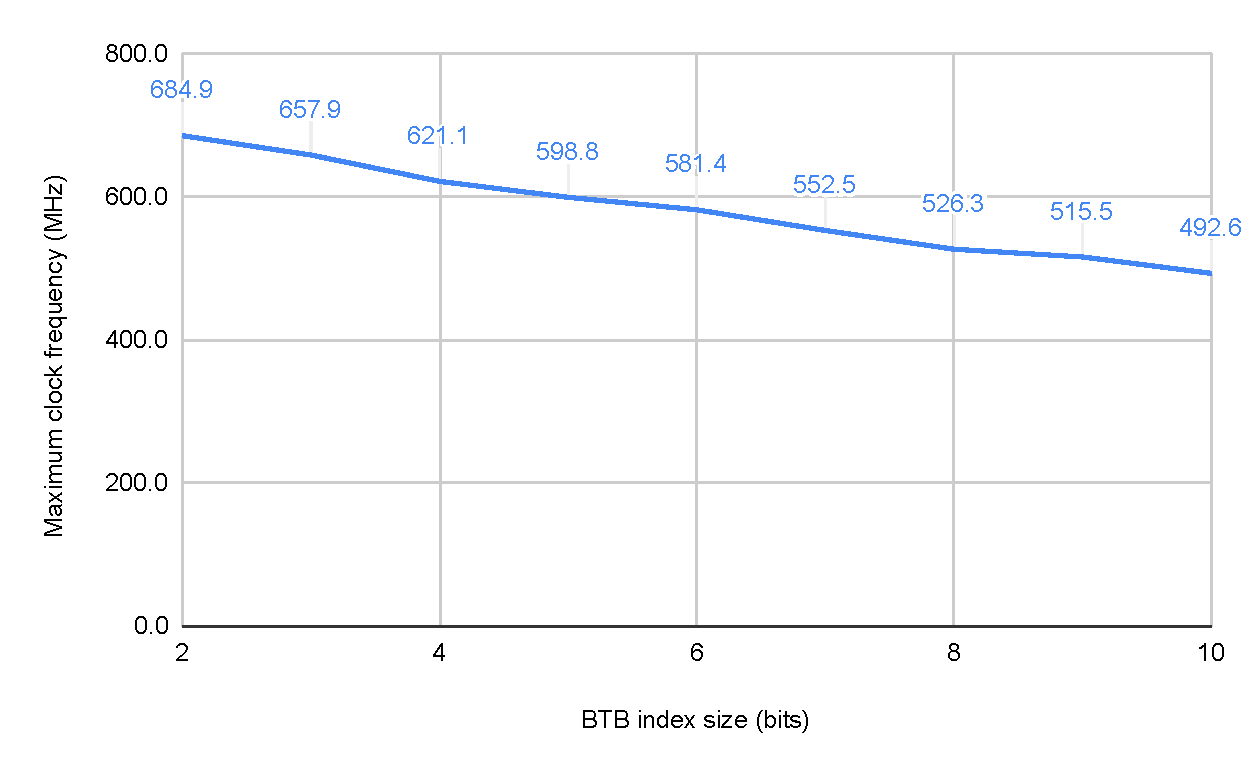
\includegraphics[width=\textwidth]{img/bpu_freq.pdf}
  \caption{Maximum \acs{BPU} clock frequency versus \ac{BTB} index bits}
  \label{fig:bpu_freq}
\end{figure}
\Cref{fig:bpu_freq} shows the results of the maximum achievable clock frequency, obtained by setting the target clock period to zero, with increasing \ac{BTB} index bits used. Between the two extremes, the critical path grows of about \SI{0.6}{ns}, which correspond to a non-negligible drop of about \SI{200}{MHz} in maximum frequency. The seemingly linear negative trend can be explained by reckoning that the decode network to address the \ac{BTB} is likely to be implemented as a balanced tree of logic gates, whose number of levels thus depends on the base-2 logarithm of the number of entries of the buffer, which in turn grows exponentially with the number of bits, leading to a linear dependence.

In the end, the actual size of the \ac{BTB} must be chosen by keeping into account the design constraints both in terms of area budget and of target clock frequency, trading them off with the prediction accuracy and hit rate. History bits, on the other hand, do not influence timing at all.

\pagebreak
\subsection{Frontend}
Given the considerations of the previous section, the entire frontend was then synthesized using 8 bits for both the \ac{BPU} history length and the \ac{BTB}, in order to have a configuration of average complexity. \Cref{tab:frontend} summarizes the results.

\begin{table}[hbt]
  \centering
  \begin{tabular}{lll}
    \toprule
                                & \textbf{BPU only}           & \textbf{Whole frontend}     \\ \midrule
    \textbf{Area}               & \SI{433233}{\micro\meter^2} & \SI{451526}{\micro\meter^2} \\ \midrule
    \textbf{Maximum frequency}  & \SI{540}{MHz}               & \SI{537}{MHz}               \\
    \bottomrule
  \end{tabular}
  \caption{Comparison of BPU and frontend synthesis results}
  \label{tab:frontend}
\end{table}

It is evident that the \ac{BPU} is by far the limiting element of the frontend, both in terms of area and timing. Given its large data structures, the surrounding logic of the rest of the frontend becomes almost negligible and represents only 4\% of the total area for this parameter configuration.

The same can be concluded for timing, as the decoding of the \ac{BTB} is unfortunately the critical path even in the whole frontend, which leads to almost the same clock frequency in both situations.

\pagebreak
To solve this issue, which could really hinder the performance of the entire design, a better implementation, as mentioned before, would employ a SRAM memory with optimized decoding networks instead of a slow large register file. This synthesis must be then only considered as indicative and preliminary, because more advanced tools and compilers could lead to better results.

On a final note, the fact that the instruction selector multiplexer could become quite large with many cache instructions per line, as anticipated in \cref{sec:instrsel}, does not incur any issue. This is because this multiplexer grows linearly with the width of the cache line, so its effect is completely masked by the exponential growth of the \ac{BPU} structures.
